% Template for PLoS
% Version 1.0 January 2009
%
% To compile to pdf, run:
% latex plos.template
% bibtex plos.template
% latex plos.template
% latex plos.template
% dvipdf plos.template

\documentclass[12pt]{article}

\usepackage{longtable}
% amsmath package, useful for mathematical formulas
\usepackage{amsmath}
% amssymb package, useful for mathematical symbols
\usepackage{amssymb}

% graphicx package, useful for including eps and pdf graphics
% include graphics with the command \includegraphics
\usepackage{graphicx}

% cite package, to clean up citations in the main text. Do not remove.
\usepackage{cite}

\usepackage{color} 
\newcommand{\hilite}[1]{\colorbox{yellow}{#1}}

% Use doublespacing - comment out for single spacing
\usepackage{setspace} 
\doublespacing


% Text layout
\topmargin 0.0cm
\oddsidemargin 0.5cm
\evensidemargin 0.5cm
\textwidth 16cm 
\textheight 21cm

% Line numbers
\usepackage{lineno}
\linenumbers

% Bold the 'Figure #' in the caption and separate it with a period
% Captions will be left justified
\usepackage[labelfont=bf,labelsep=period,justification=raggedright]{caption}

% Use the PLoS provided bibtex style
\bibliographystyle{plos2009}

% Remove brackets from numbering in List of References
\makeatletter
\renewcommand{\@biblabel}[1]{\quad#1.}
\makeatother


% Leave date blank
\date{}

\pagestyle{myheadings}
%% ** EDIT HERE **


%% ** EDIT HERE **
%% PLEASE INCLUDE ALL MACROS BELOW

%% END MACROS SECTION

\begin{document}

% Title must be 150 characters or less
\begin{flushleft}
{\Large
\textbf{Biases in the Experimental Annotations of Protein Function and their Effect on Our
Understanding of Protein Function Space}
}
% Insert Author names, affiliations and corresponding author email.
\\
\author{Alexandra Schnoes$^1$%
       \email{Alexandra Schnoes - alexandra.schnoes@ucsf.edu}%
         David C. Ream$^2$%
         \email{David Ream - reamdc1@miamioh.edu}
      \and
         Alexander Thorman$^2$%
         \email{Alexander Thorman - thormanaaw@muohio.edu}
      \and
         Patricia Babbitt$^1$%
         \email{Patricia Babbitt - babbittp@ucsf.edu}
       \and 
        Iddo Friedberg\correspondingauthor$^{2,3}$%
        \email{Iddo Friedberg\correspondingauthor - i.friedberg@miamioh.edu}
      }
      

%Author1$^{1}$, 
%Author2$^{2}$, 
%Author3$^{3,\ast}$
%% \address{
%%    \iid(1)Department of Bioengineering and Therapeutic Sciences, University of California San Francisco, 
%%            San Francisco, CA, USA\\
%%      \iid(2)Department of Microbiology, Miami University, Oxford, OH USA\\
%%      \iid(3)Department of Computer Science and Software Engineering , Miami University, Oxford, OH USA
%% }%
\bf{1} Alexandra Schnoes Dept/Program/Center, University of California, San Francisco, San Francisco, CA,
USA
\\
\bf{2} David C. Ream Department of Microbiology, Miami University, Oxford, OH, USA
\\
\bf{3} Alexander W. Thorman, Department of Microbiology, Miami University, Oxford, OH, USA
\\
\bf{4} Patricia C. Babbitt Dept/Program/Center, University of California, San Francisco, San Francisco, CA,
USA
\\
\bf{5} Iddo Friedberg, Department of Microbiology and Computer Science \& Software engineering, Miami University, Oxford, OH, USA
\\
$\ast$ E-mail: corresponding i.friedberg@muohio.edu
\end{flushleft}

% Please keep the abstract between 250 and 300 words
\section*{Abstract}

        \paragraph*{Background:} Computational protein function
prediction programs rely upon well-annotated databases for testing and training
their algorithms. These databases, in turn, rely upon the work of curators
to capture experimental findings from scientific literature and apply them to protein
sequence data. However, with the increasing use of high-throughput experimental
assays,  a small number of experimental articles dominate
the functional protein annotations collected in databases. 
Here we investigate just how prevalent is the ``few articles --
many proteins'' phenomenon. We hypothesize that the dominance of high-throughput experiments in
proteins annotation biases our view of the corpus of functions enabled by proteins.
      
        \paragraph*{Results:} We examine the annotation of
UniProtKB by the Gene Ontology Annotation project (GOA), and show that
the distribution of proteins per article is a log-odd, with 0.06\% of articles
dominating 20\% of the annotations. Since each of the dominant articles
describes the use of an assay that can find only one function or a small
group of functions, this leads to substantial biases, in several aspects, in what we know
about the function of many proteins.

        \paragraph*{Conclusions:} Given the experimental techniques
available, protein function annotation bias due to high-throughput experiments is unavoidable. Knowing
that these biases exist and understanding their characteristics and extent is important for
database curators, developers of function annotation programs, and
anyone who uses protein function annotation data to plan experiments.

% Please keep the Author Summary between 150 and 200 words
% Use first person. PLoS ONE authors please skip this step. 
% Author Summary not valid for PLoS ONE submissions.   
\section*{Author Summary}

\section*{Introduction}

Functional annotation of proteins is a primary challenge in molecular biology
today\cite{Friedberg2006Automated, Erdin2011180, Rentzsch2009210, Fetrow2012}. The ongoing
improvements in sequencing technology had the emphasis shifting from realizing the \$1000 genome to
the 1-hour genome \cite{PMID Stahl2012Toward}. The ability to rapidly and cheaply sequence genomes
is creating a flood of sequence data, which require extensive analysis and characterization before
these data can be useful. A large proportion of this work involves assigning biological function to
newly determined gene sequences, a process that is both complex and costly \cite{Sboner2011Real}.
Furthermore,  the ability to accurately assign function through computational means is challenging
and open problem \cite{Schnoes2009Annotation}. To aid current annotation procedures and improve
computational function prediction algorithms, sources of high-quality, experimentally derived
functional data are necessary. Currently, one of the few repositories of such data is the
UniProt-GOA database \cite{Dimmer2012UniProtGO}, which contains both computationally derived and
literature derived functional information. The literature derived information is extracted by human
curators who capture functional data from publications, assign the data to its appropriate place in
the Gene Ontology hierarchy \cite{Ashburner2000Gene} and label them with appropriate functional
evidence codes. The UniProt-GOA database is one of only a small number of databases that explicitly
connects functional data, publication references and evidence codes to specific, experimentally
studied sequences.  In addition, annotations captured in UniProt-GOA directly impact the
annotations in the UniProt/Swiss-Prot database, widely considered to be a gold standard set of
functional annotation \cite{Schnoes2009Annotation}. 

It is therefore important to understand any trends and biases that are
encapsulated by the UniProt-GOA database, as those impact well-used sister
databases and therefore a large number of users worldwide. Furthermore,
any biases would impact function prediction algorithms development and training.

One concern surrounding the capture of functional data from articles is the propensity for
high-throughput experimental work to become a large fraction of the data in UniProt-GOA,
thus having few experiments dominate the protein function landscape. In this work we
analyzed the relative contribution of articles to the experimental annotations in UniProt-GOA.
We found some striking biases, stemming from the fact that a small fraction of articles that
describe high-throughput experiments disproportionately contribute to the pool of
experimental annotations of model organisms. Consequently, we show that: 1) annotations
coming from high-throughput experiments are mostly less informative than those provided by
low-throughput experiments;  2) annotations from high throughput experiments bias the
annotations towards a limited number of functions, and, 3) many high-throughput experiments
overlap in the proteins they annotate, and in the annotations assigned. Taken together, our
findings offer a comprehensive picture of how the current protein function landscape is
generated. Furthermore, due to the biases inherent in the current system of sequence
annotations, this study serves as a caution to the producers and consumers of biological data
from high-throughput experiments. 


% Results and Discussion can be combined.
\section*{Methods and Results}


\subsection*{Articles and Proteins} With the advent of high-throughput experiments it has become
possible to conduct large-scale studies of protein functions.  Consequently, some studies reveal
very specific functional aspects of a large amount of proteins as a result of the particular type
of assay or assays used. To understand the impact of large-scale studies on the corpus of
experimentally annotated proteins, we looked at the UniprotKB Gene Ontology (GO) annotation files,
or UniProt-GOA. UniProt-GOA proteins are individually annotated by one or more GO terms using a
procedure described in \cite{Dimmer2012UniProtGO}. Briefly, this procedure consists of six steps
which include sequence curation, sequence motif analyses, literature-based curation, reciprocal
BLAST\cite{Altschul1997Gapped} searches, attribution of all resources leading to the included
findings, and quality assurance. If the annotation source is a research article, the attribution
includes its PubMed ID. For each GO term associated with a protein, there is also an
\textit{evidence code} (EC) which is used to explain how the association between the protein and
the GO term was made.  Experimental evidence codes include such terms as: Inferred by Direct Assay
(IDA) which indicates that ``a direct assay was carried out to determine the function, process, or
component indicated by the GO term'' or Inferred from Physical Interaction (IPI) which ``Covers
physical interactions between the gene product of interest and another molecule.'' (All EC
definitions were taken from the GO site, geneontology.org).  Computational evidence codes include
terms such as \textit{Inferred from Sequence or Structural Similarity} (ISS) and \textit{Inferred
from Sequence Orthology} (ISO).  Although the evidence is non-experimental, the proteins annotated
with these evidence codes are still assigned by a curator, rendering a level of human oversight.
There are also non-computational and non-experimental evidence codes, the most prevalent being
\textit{Inferred from Electronic Annotation} (IEA) which is ``used for annotations that depend
directly on computation or automated transfer of annotations from a database''. IEA evidence means
that the annotation was not made or checked by a person.  Different degrees of reliability are
associated with the evidence codes, with experimental codes generally considered to be of higher
reliability than non-experimental codes.  However, the increase in the number of high-throughput
experiments used to determine protein functions may introduce biases into experimental protein
annotations, due to the inherent capabilities and limitations of high-throughput assays.  To test
the hypothesis that such biases exist, and to study their extent if they do, we compiled the
details of all experimentally-annotated proteins in UniProtKB. This included all proteins whose GO
annotations have the GO experimental evidence codes EXP, IDA, IPI, IMP, IGI, IEP. We first examined
the distribution of articles by the number of proteins they annotate. 
As can be seen in Figure~\ref{fig:articles-prots}, the distribution of the number of proteins
annotated per article follows a power-law distribution. $f(x)=a\dot x^k$.  Using linear regression
over the log values of the axes we obtained a fit with $p<1.18\times 10^8$ and $R^2=-0.72$.  We
therefore conclude that there is indeed a substantial bias in experimental annotations, in which
there are few articles that annotate a large number of proteins.

To better understand the consequences of such a distribution, we divided the annotating articles
into four cohorts, based on the number of proteins each article annotates.
\textit{Single-throughput} articles are those articles that annotate only one protein; \textit{low
throughput} articles annotate 2-9 proteins; \textit{moderate throughput} articles annotate 10-99
proteins and \textit{high throughput} articles annotate over 99 proteins. The results are shown in
Table~\ref{tab:cohorts}. The most striking finding is that high throughput articles are responsible
for 25\% of the annotations in Uniprot-GOA, even though they comprise 0.08\% of the articles. 96\%
of the articles are single-throughput and low throughput, however those annotate only 53\% of the
proteins in Uniprot-GOA. So while moderate throughput and high-throughput experiments account for
almost half of the annotations in Uniprot-GOA, they comprise only 4\% of the experiments
published.

What typifies high-throughput articles? Also, how may the log-odds distribution bias what we
understand of the protein function universe? To answer these questions, we examined
different aspects of the annotations in the four article cohorts. Also, we examined in higher
detail the top 50 annotating articles. (Overall, 62 articles in our study annotated more than
100 proteins). 
An initial characterization of the top 50 high-throughput articles is shown in
Table\ref{table:top-articles}. As can be seen, all of the articles are specific to a
single species (typically a model organism) and assay that is used to annotate the proteins
in that organism.  Since a single assay was used, then typically only one ontology (MFO, BPO
or CCO) was used for annotation. For some species this means that a single functional aspect
(MFO, BPO or CCO) of a species will be dominated by a single experiment.

\subsection*{Term frequency bias}
To see how much a single species-- and method-- specific high-throughput assay affects the entire
annotation of a species, we examined the relative contribution of the top-50 articles to the entire
corpus of experimentally annotated protein in each species.  All the species found in the top-50
articles were either common
model organisms or human.
For each species, we looked at the five most frequent terms in the top 50 annotating articles. We then
examined the contribution of this term by the top 50 articles to the general annotations of that
species.  The \textit{contribution} is the number of annotations by any given GO term in the top 50
articles divided by the number of annotations by that GO term in all of UniProtKB.  For example, as
seen in Figure~\ref{fig:rel-contrib} in \textit{D.  melanogaster} 88\% of the usage of
``precatalytic splicosome'' is contributed by the top-50 articles. 

% "Annotation Trends" in Alex's poster

For most organisms in the top-50 articles,  the annotations were within the cellular component
ontology. The exceptions are \textit{D. melanogaster} and \textit{C. elegans} where the
dominant terms were from the Biological Process ontology, and in mouse, where ``protein
binding'' and ``identical protein binding'' are from the Molecular Function Ontology.
\textit{D. melanogaster}'s annotation for the top terms is dominated (over 50\% contribution)
by the top-50 articles. 

The term frequency bias described here can be viewed more broadly within the ontology bias. The
proteins annotated by the cohorts of single-protein articles, low-throughput articles, and moderate throughput
articles have similar ratios of the fraction of proteins annotated.  Twenty-two to twenty-six
percent of assigned terms are in the Molecular Function Ontology, and 51-57\% are in the
Biological Process Ontology and the remaining 17-25\% are in the Cellular Component ontology.
These ratios change dramatically with high-throughput articles (over 99 terms per article). In the
high-throughput articles, only 5\% of assigned terms are in the Molecular Function Ontology, 38\%
in the Biological Process Ontology and 57\% in the Cellular Compartment Ontology, ostensibly due
to a lack of high-throughput assays that can be used for generating annotations using the
Molecular Function Ontology. 

% The next paragraph should be should be moved to Methods. We'll just write that we removed the
% propagation bias. This is not a finding, it's a technical clean-up.
% EDIT EDIT: probably can do without this finding.
%Another type of annotation bias may result due to GO-structure derived redundancy: the annotation of
%a single term using a given GO-term and one or more of its parents. However, this type of
%annotation may not necessarily be wholly redundant. For example, a protein may localize to
%the nucleolus and the nucleus itself. In the Cellular Compartment ontology, ``nucleus'' is
%a parent term for ``nucleolus''. In the case of this hypothetical protein, annotating with
%``nucleolus'' and ``nucleus'' is not an error. However, if the protein was found to
%localize to the nucleolus only, then annotating with both terms is a redundancy. We termed
%such a redundancy \textit{propagation bias}. We examined all proteins for possible propagation
%bias. If a protein was annotated with a GO term and one or more parent terms, the parent
%terms were removed. We found possible propagation biases in 17 of the 50 articles. The results
%are summarized in Table\ref{tab:prop-bias}. 

\subsection*{Reannotation Bias}

% Text for dream-catcher plots
Another type of annotation bias is that of protein re-annotation. How many of the top-50 articles
actually re-annotate the same set of proteins? And how much of an agreement is there between
different experiments?  To investigate the extent of repetitive annotations in different articles, we
clustered all the proteins annotated by the top-50 articles using CD-HIT\cite{CD_HIT} at 100\%
sequence identity. We then examined the number of clusters containing 100\% identical sequences per
model species. The product of the number of proteins divided by the number of clusters is the
redundancy percentage. For example, if each of the top-50 articles annotating the proteins in a given
species annotated the same protein set, the redundancy percentage would be 100\%. The results of
the reannotation bias analysis are shown in Figure~\ref{fig:dreamcatcher1} and in
Table~\ref{tab:dreamcatcher1}. As can be seen, the highest redundancy (65\%) is in the 12 articles
annotating \textit{C. elegans}. 
% However, when normalized by number of annotating articles, the highest
% redundancy is found in Mouse (15.33\% in three articles) closely followed by \textit{M. tuberculosis}
% (14\% in two articles). Taken together, these results show that there is repetition in the annotation
% of proteins in most model organisms using high-throughput assays, although that redundancy varies.


We have determined therefore, that there is a varying degree of repetition between
experiments in the proteins they annotate, with some overlaps being quite high. In those
cases, many of the same proteins in the same organism are being annotated. However, there
is still a need to determined whether this annotation is consistent or not. To do this, we
looked for the proteins that are annotated by more than one article, within the same
ontology.

Given a protein $P$, let $G$ be the GO-terms $g_1,g_2,\dots,g_m$ that annotate that protein
in all top-50 articles for an ontology $O \in \{BPO,MFO,CCO\}$. The count of each of these
go terms per protein per ontology is $n_1,n_2,\dots,n_m$ with $n_i$ being the number of
times GO term $g_i$ annotates protein $P$.

The number of total annotations for a protein in an ontology is $\sum_1^m n_i$ . The
\textit{maximum annotation consistency} for protein $P$ in ontology $O$ $0 \leq k_{P,O}
\leq 1$ is calculated as:

\[
k_{P,O} = \frac{max(n_1,n_2,\dots,n_m)}{\sum^m n_i} for max(n_1,n_2,\dots,n_m) \geq 2
\]


For example, the protein Oleate activated transcription factor 3 (UniProtID: P36023) in \textit{S.
cerevisiae} is annotated by three articles in the CC ontology:

\begin{table}
\begin{tabular}{l l l l l}
PubMedID  &  UniProt ID& Ontology & GO-term & description \\
14562095  &  P36023    & CCO & GO:0005634  &   nucleus \\
14562095  &  P36023    & CCO  &  GO:0005737 &  cytoplasm \\
16823961  &  P36023    & CCO  & GO:0005739  &    mitochondrion \\
14576278  &  P36023    & CCO  & GO:0005739  &    mitochondrion \\
\end{tabular}
\end{table}

The annotation consistency for P36023 is therefore the maximum count of identical GO terms
(\textit{mitochondrion}, 2), divided by the total number of annotations, 4: 0.5.

Table~\ref{tab:dreamcatcher2} shows the results of this analysis. In \textit{A. thaliana},
1941 proteins are annotated by 15 articles and 18 terms in the Cellular Component ontology.
The mean maximum-consistency is 0.251. The highest mean consistency is for the annotation
of 807 mouse proteins annotated in Cellular Component ontology with an annotation
consistency 0.832. However, that is not surprising given that there are only three
annotating articles, and two annotating terms. We omitted the ontology and organism
combinations that were annotated by less than three articles or two GO terms, or both.

\subsection*{Quantifying annotation information}

A common assumption holds that while high-throughput experiments do annotate more protein
functions than low-throughput experiments, the former also tend to be more shallow in the
predictions they provide. The information provided, for example, by a large-scale protein
binding assay will only tell us if two proteins are binding, but will not reveal whether
that binding is specific, will not provide an exact $K_{bind}$, will not say under what
conditions binding takes place, or whether there is any enzymatic reaction or
signal-transduction involved. Having on hand data from experiments with different
``thorughputness'' levels,  we set out to investigate whether there is a difference in the
information provided by high-throughput experiments vs. low-throughput ones. To answer this
question, we first had to quantify the information given by GO terms. One way to do so, is
to use the depth of the term in the ontology: the term ``enzyme activity'' would be less
informative than ``dehalogenase'' and the latter will be less informative than ``haloalkane
dehalogenase''.  We therefore counted edges from the ontology root term to the GO-term to
determine term information. The larger the number of edges, the more specific -- and
therefore informative -- the annotation. In cases where several paths lead from the root to
the examined GO-term, we used the minimal path. We did so for all the annotating articles
split into groups by the number of proteins each article annotates. 

Edge counting provides a measure of term-specificity. It is, however, imperfect. The reason is
that different areas of the GO DAG have different connectivities, and terms may have different
depths unrelated to the intuitive specificity of a term. For example ``high-affinity Tryptophan
transporter'', (GO:0005300) is 14 terms deep, while ``anticoagulant'', (GO:0008435) is only three
terms deep.  For this reason, information content, the logarithm of the inverse of the GO term
frequency in the corpus is generally accepted as a measure of GO-term information
content\cite{lord-semsim}. To account for the possible bias created by the GO-DAG structure, we
also used the log-frequency of the terms in the experimentally annotated proteins in Uniprot-GOA.
However, it should be noted that the log-frequency measure is also imperfect because, as we see
throughout this study, a GO-term's frequency may be heavily influenced  by the top annotating
articles, injecting a circularity problem into the use of this metric. Since no
single metric for measuring the information conveyed by a GO term is wholly satisfactory, we used
both in this study.

The results of both analyses are shown in Figure~\ref{fig:go-depth} %and the accompanying
%Table~\ref{tab:go-depth}. 
In general, the results from the depth-based analysis and the
log-frequency based analysis are in agreement, when compared across groupings based on the
number of proteins annotated by the articles. For the Molecular Function ontology, the
distribution of edge counts and log-frequency scores decreases as the number of annotated
proteins per-article increases.  For the Biological Process ontology, the decrease is
significant. However the contributer to the decrease are the high-throughput articles
while there is little change in the first three article cohorts.
Finally, there is no significant trend of GO-depth decrease in the Cellular Component
Ontology. However, using the information content metric, there is also a significant decrease
in information content in the high-throughput article cohort.


\subsection*{Evidence and Assertion}

There are two complementary ways by which we come to knowledge about a protein's function.
The twenty evidence codes, discussed above, encapsulate the type results by which the
function was inferred, but they do not capture all the necessary information. For example,
``Inferred by Direct Assay (IDA)'' informs that experimental evidence was used, but does
not say which type of experiment was performed.  This information is often needed, since
knowing which experiments were performed can help the researcher establish the reliability
and scope of the data. For example, RNA used in an  RNAi experiment does not traverse the
blood-brain-barrier, meaning that no data from the central nervous system can be drawn from
an RNAi experiment. The Evidence Code Ontology, or ECO, seeks to improve upon the
GO-attached evidence codes. ECO provides more elaborate terms than ``Inferred by Direct
Assay'': ECO also conveys which assay was used, i.e.  ``microscopy'', ``RNA interference''
etc.  In addition to evidence terms, the ECO ontology provides \textit{assertion terms} in
in which the nature of the assay is given. For example, an enzyme-linked immunosorbent
assay (ELISA) provides quantitative protein data \textit{in vitro} while an immunogold
assay may provide the same information, and cellular localization information \textit{in
vivo}. It is therefore important to know both the assertion and the evidence to understand
what sort of information may be gleaned from the assay. However, to understand which types
of assertions are made in the top-50 high throughput articles, we manually assigned
Evidence Codes Ontology (ECO) assertion and evidence terms to the top-50 articles. The ECO
ontology is more elaborate than the evidence codes used by Uniprot-GOA.  Although there are
plans to insert ECO terms into Uniprot-GOA in the near future, those will probably not be
done manually for proteins already existing in Uniprot-GOA, but by automatic mapping EC
terms to ECO ontology terms using a preset table (Rachael Huntley, Chris Mungall  and Tony
Sawford, personal communication). Thus, the ECO-based annotations we provide here to the
top 50 articles is probably more informative than a future annotation may provide.

The results are shown in Figure~\ref{fig:assertion} and in
Table~\ref{tab:assertion}.

Interestingly, the most third most-frequently used assertion in the top experimental
articles was not an experimental assertion, but rather a computational one: the term
ECO:00053 ``computational combinatorial evidence'' is defined as ``A type of combinatorial
analysis where data are combined and evaluated by an algorithm.'' This is not a
computational prediction per-se, but rather a combination of several experimental lines of
evidence used in a article.

The most used experimental assertion term was ECO:000160 ``protein separation followed by fragment
identification evidence'', which encompasses different types of mass-spectrometry experiments. The
next ranking assertion terms were computational: ``motif similarity evidence'' and ``sequence
similarity evidence used in automatic assertion''. Those were generally combined with the
mass-spectrometry experiments to identify protein sequence fragments reconstructed from the
mass-spectrometry. Another frequently used experimental techniques was ``RNAi experimental
evidence''. This type of experiment was mostly with the articles that used RNA interference in
studying \textit{C. elegans}, whose study comprised 12 of the top-50 articles.

% \subsection*{Annotation quality}
% 
% One reflection on annotation coverage is the number of GO terms assigned to any
% given protein. Ostensibly, the larger the number of GO terms that are assigned to a
% protein, the more comprehensive its annotation, provided that these terms are
% non-redundant, i.e. not direct parents of each other. 
% 
% The median number of annotations per protein was 1.09, which means that most of the top-50
% articles do not provide more than a single GO-term per protein. Also, the mean number of
% annotations per protein was 1.59. The difference between the mean and median reflects that
% most articles have an annotations-per-protein ratio which is close to 1, whereas few have a
% higher annotation ratio. As shown in Figure~\ref{fig:annotation-ratio}, that is essentially
% the case. Seven articles had an annotations per proteins ratio which is above 2. Those
% were article numbers 1, 4, 10, 23, 34 and 43 on the list. We decided to examine these articles
% to see whether these studies did indeed provide better coverage, and what distinguished them
% from the other high throughput studies. To follow are brief summaries of the
% methodologies used in these articles.
% 
% \textbf{Toward a confocal subcellular atlas of the human proteome.}
% 
% In this microscopy-based study, the authors used specific staining techniques and confocal
% microscopy to describe the subcellular localization of 4937 proteins, which were each assigned
% to one or more of ten different subcellular compartments. Since proteins may be assigned to more
% than a single compartment, there is a mean of 2.23 GO annotations per protein. The most frequent
% terms were ``nucleus'' and ``cytosol'' with 2211 and 2208 terms, respectively. The next
% most frequent terms was``cytoplasm'', ``endoplasmatic reticulum'' and ``golgi apparatus'' with
% 400-500 terms each.  ''\cite{PMID:11121744}. This article is the top annotating one that we found,
% both in GO-terms per protein, and in total number of proteins annotated. 
% 
% \textbf{RNAi-based studies of \textit{C. elegans}}
% 
% In \cite{PMID:17417969} the authors fed various bacterial clones expressing dsRNA to \textit{C.
% elegans} mutants that are hypersensitive to dsRNA interference. As  a result, they discovered
% novel loss-of-function phenotypes for 393 \textit{C. elegans} genes. In total they reported 5918
% annotations for 1791 proteins.  The functions reported herefact, ere for the Biological Process
% Ontology. Figure 2B 
% 
% The three other studies were also RNAi-based using \textit{C. elegans}. 


\section*{Discussion}

We have identified several annotation biases in UniProt-GOA. These biases stem from the
uneven number of annotations produced by different types of experiments. It is clear that
results from high-throughput experiments contribute substantially to the function annotation
landscape, as up to 20\% of experimentally annotated proteins are annotated by
high-throughput assays, with most of them not being annotated by medium-- or
low--\~throughput experiments. 

At the same time, high throughput experiments produce less information per protein than
moderate--, low-- and single--\~throughput experiments as evidenced by the type of terms
produced in the Molecular Function and Biological Process ontologies. Furthermore, the
number of total GO terms used in the high-throughput experiments is much lower than that
used in low and medium throughput experiments. Therefore, while high throughput experiments
provide a high coverage of protein function space, it is the low throughput
experiments that provide more specific information, as well as a larger diversity of terms.

We have also identified several types of biases that are contributed by high throughput
experiments.  First, there is the enrichment of low-information content GO-terms, which
means that our understanding of the protein function as provided by high throughput
experiments is limited.  Second, there is the small number of terms used, when considering
the large number of proteins that are being annotated. Third is the general term bias
towards the cellular component ontology and, to a lesser extent, the Biological Process
ontology; at the same time, there are very few articles that deal with the Molecular
Function ontology.  These biases all stem from the inherent capabilities and limitations of
the hight-throughput experiments.  A fourth, related bias is the organism studied: taken
together, \textit{C. elegans} and \textit{A. thaliana} studies comprise 36 (72\%) of the
top-50 annotating articles. 

The most frequent experiment performed is cell fractionation and mass-spectrometry to
assign a Cellular Component ontology terms (citations).  Consequently this means that the
assignment procedure is limited to the cellular compartments that can be identified with
the fractionation methods used\cite{MS-articles}. So while Cellular Component is the most
frequent annotation used, mass-spectrometry is the most common method used to localize
proteins in subcellular compartments. A notable exception to the use of MS for protein
localization is in the top annotating article \cite{pmid18029348} which uses microscopy for
subcellular localization. The only MS experiment in the top-50 articles whose proteins were
not annotated with cellular localization was ``Proteome survey reveals modularity of the
yeast cell machinery''\cite{pmid18029348}. The resulting annotation was ``protein binding''
form the Molecular Function ontology. A more detailed discussion on this study follows in
the section \textbf{Information Capture} below.

The second most frequent type of experiments used RNA Interference (RNAi) whole-genome gene
knockdowns in \textit{C. elegans}, \textit{D. melanogaster} and one in \textit{C. albicans}.
RNAi experiments typically use targeted dsRNA which is delivered to the organism and silences
specific genes. Typically the experiments here used libraries of RNAi targeted to the whole
exome. The phenotypes searched for were mostly associated with embryonic and post-embryonic
development \cite{relevant articles}. Some studies focused on mitotic spindle
assembly\cite{pmid17412918}, lipid storage\cite{pmid17412918} and endocytic
traffic\cite{pmid17412918}. One study used RNAi and MP to identify mitochondrial protein
localization \cite{pmid18433294}.

These two types of assays (mass-spectrometry and RNAi)  were strongly linked to the other
frequently used experimental ECO terms, by the nature of the methodology used. Thus, ``protein
separation followed by fragment identification evidence'' is usually accompanied with ``cell
fractionation evidence'' and ``Western blot evidence''. ``RNAi experimental evidence'' is
generally associated with ``mutant phenotype evidence used in manual assertion''. All experiments
are associated with computational ECO terms, which describe sequence similarity and motif
recognition techniques used to identify the sequences found. Thus, a strong reliance on
computational annotation is an integral part of high throughput experiments. It should be noted
that computational annotation here is not necessarily used directly for functional annotation,
but rather for identifying the protein by a sequence or motif similarity search.

\subsection*{Information Capture and Scope of GO}

We have discussed the information loss that is characteristic of high-throughput
experiments, due to the nature of these experiments. However, another reason for information loss
is the inability to capture certain types of information using the Gene Ontology. GO is knowingly
limited to three aspects (MF, BP and CC) of biological function, which are assigned per protein.
However, other aspects of function may emerge from experiments that cannot be captured by GO.  Of
note is the study mentioned earlier, ``Proteome survey reveals modularity of the yeast cell
machinery''\cite{pmid18029348}.  In this study, the information produced was primarily of protein
complexes, which proteins are binding which proteins, and the relationship to cellular
compartmentalization and biological networks. At the same time, the only GO-term captured in the
curation of this study was ``protein binding''.  Some, but not all of this information can be
captured more specifically using the children of the term ``protein binding'', but such a process
is arguably laborious by manual curation of a high throughput article.  Furthermore, the main
information conveyed by this article, namely the types of protein complexes discovered and how they
relate to cellular networks, is outside the scope of GO. It is important to realize that while
high-throughput experiments do convey less information per protein within the functional scope as
defined by GO, they still convey composite information such as possible pathway mappings --
information which needs to be captured into annotation databases by means other than GO.  In the
example above, the information can be captured by a protein interaction database, but not by GO
annotation.

\section*{Conclusions}

Taken together, the annotation biases noted in this study affect our understanding of
protein function space. This, in turn, affects out ability to properly understand the
connection between predictors of protein function and the actual function -- the hallmark
of computational function annotation. As a dramatic example, during the Critical Assessment
of Function Annotation experiment (Radivojac \textit{et al} in review) we have noticed that
about 20\% of the proteins participating in the challenge and annotated with the Molecular
Function Ontology were annotated as ``protein binding'', a GO-term that conveys little
information. Furthermore, it was shown that the major contribution of ``protein binding''
term to the CAFA challenge data set was due to high-throughput assays. This illustrates how
the concentration of a large number of annotations in a small number of studies provides
only a partial picture of the function of these proteins. As we have seen, the picture
provided from high throughput experiments is mainly of: 1. subcellular localization cell
fractionation and MS based localization and 2. developmental phenotypes. While these data
are important, we should be mindful of this bias when examining protein function in the
database, even those annotations deemed to be of high quality, i.e. with experimental
verification. Furthermore, such a large bias in prior probabilities can adversely affect
programs employing prior probabilities, as most machine-learning programs do. Many
researchers use programs based on machine-learning algorithms to predict the function of
unknown proteins. If the training set for these programs has included a disproportional
number of annotations by thigh-throughput experiments, the results these programs provide
will be strongly biased towards a few frequent and shallow GO-terms.

Several steps can be taken to remedy this situation. Annotations are derived from
high-throughput experiments can be flagged as such in the database. The flagging can then be
read by sequence similarity or other search software, and flagged proteins removed or
otherwise marked in the search.  In a typical scenario, a researcher will BLAST their query
protein to determine its function by sequence similarity. If a target protein is tagged as
annotated by a high throughput assay, it would be removed form the search if asked to do so
by the user. This filtering can also be done by assay type, number of proteins annotated per
experiment, or a combination of the above. This requires that GO-annotated proteins should
also be annotated with assertion codes in addition to the evidence codes and GO term-codes;
but given the large volume of data in UniprotKB is it hard to expect such massive
reannotation with assertion terms undertaken. \hilite{(Any other ideas?)}

We call upon the communities of annotators, computational biologists and experimental biologists to
be mindful of the phenomenon of the biases described in this study, and to work together to
understand its implications and mitigate its impact.


% You may title this section "Methods" or "Models". 
% "Models" is not a valid title for PLoS ONE authors. However, PLoS ONE
% authors may use "Analysis" 
%\section*{Materials and Methods}
\section*{Note on Methods}
We used the Uniprot-GOA database from December 2011. Data analyses were performed using Python scripts.
ECO terms classifying the proteins in the top 50 experiments were assigned to the proteins
manually after reading the articles. All data and scripts are available on
http://github.com/FriedbergLab/DataBias/

% Do NOT remove this, even if you are not including acknowledgments
\section*{Acknowledgments}
We thank Predrag Radivojac, members of the Friedberg and Babbitt labs for insightful discussions.
This research was funded, in part by NSF / ABI XXXXXXX-XXX award to IF and XXXXXXXXXXXX to PCB.

\section*{References}
% The bibtex filename
\bibliography{sp_bias.bib}
\newpage
\section*{Figures}
%\begin{figure}[!ht]
%\begin{center}
%%\includegraphics[width=4in]{figure_name.2.eps}
%\end{center}
%\caption{
%{\bf Bold the first sentence.}  Rest of figure 2  caption.  Caption 
%should be left justified, as specified by the options to the caption 
%package.
%}
%\label{Figure_label}
%\end{figure}

\begin{figure}[!ht]
\begin{center}
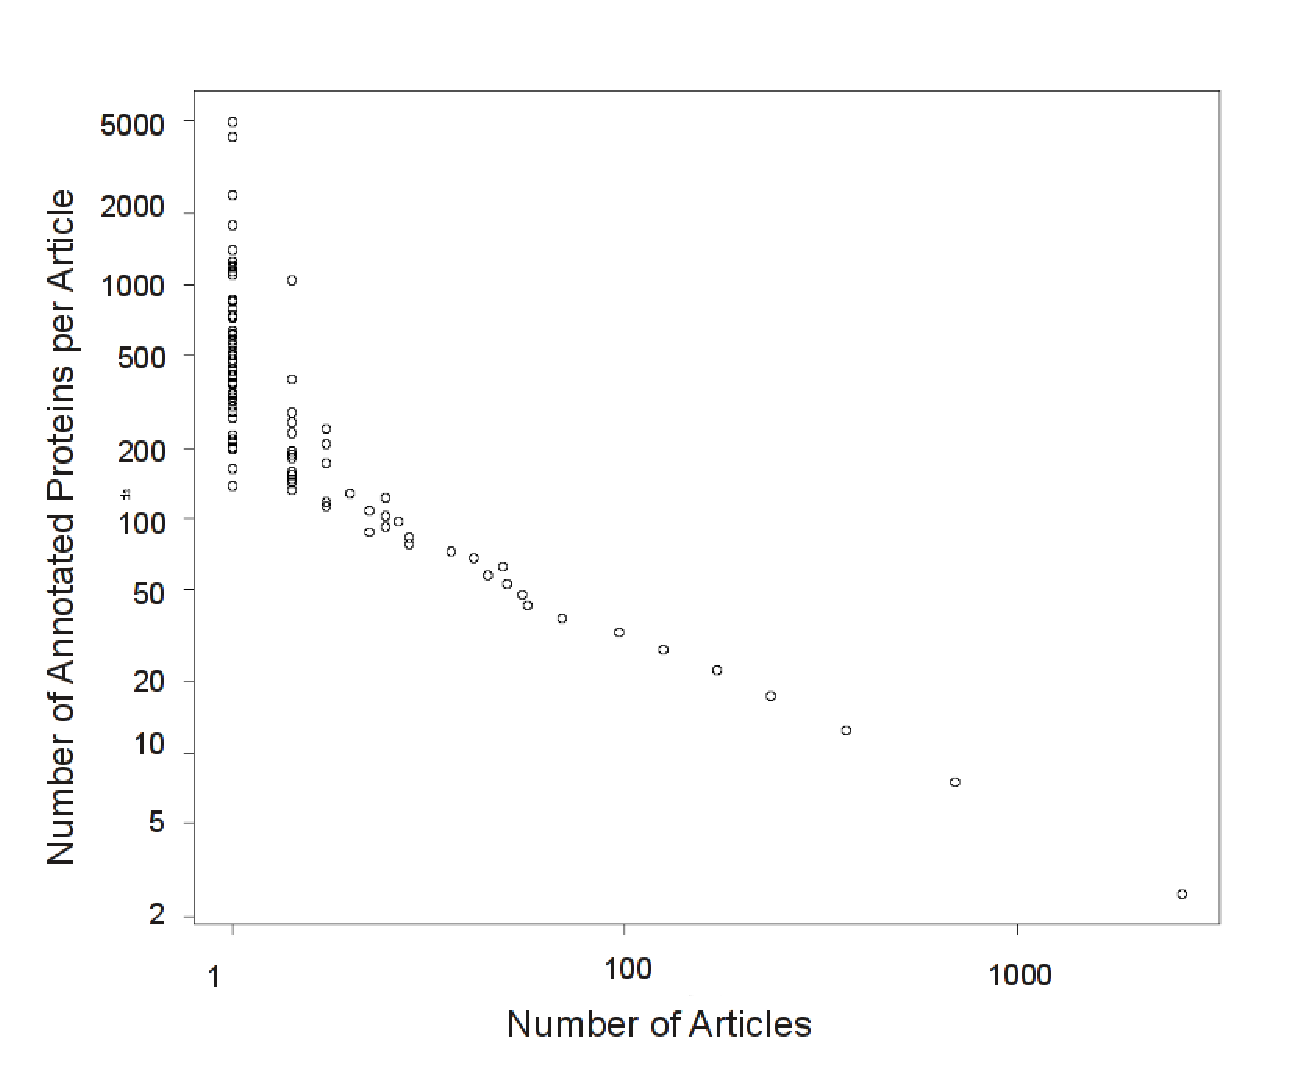
\includegraphics[width=6in]{articles-prots.eps}
\end{center}
\caption{
{\bf Distribution of the number of proteins annotated per article.} X-axis: number of annotating
articles. Y-axis: number of annotated proteins. The distribution was found to be logarithmic with a
significant ($R^2=0.72; p<1.10\times 10^{18}$) linear fit to the log-log plot. The data came from 76137
articles annotating 256033 proteins with GO experimental evidence codes, in Uniprot-GOA 12/2011.
}
\label{fig:articles-prots}
\end{figure}
\newpage

\begin{figure}[!ht] 
\begin{center} 
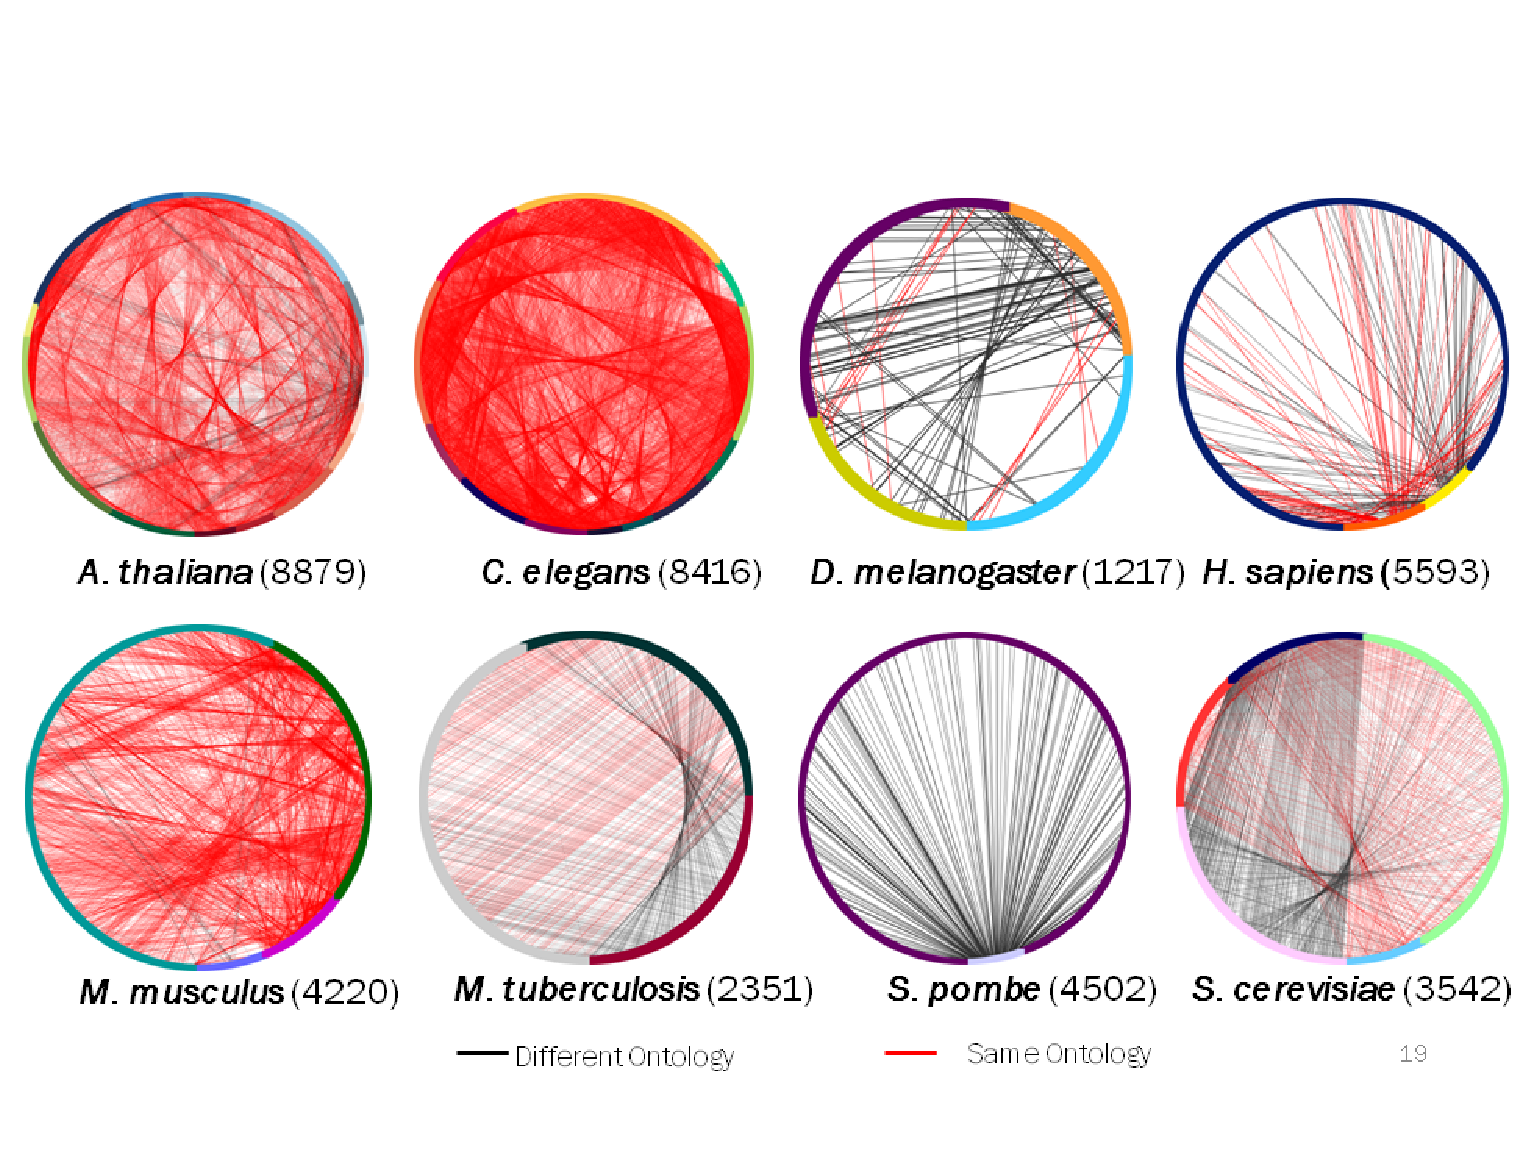
\includegraphics[width=7in]{dreamcatcher1.eps} 
\end{center}
\caption{ {\bf Redundancy in proteins described by the top-50 articles.} A circle represents the sum
total of articles annotating each organism. Each colored arch is composed of all the proteins in a
single article. A line is drawn between any two points on the circle if the proteins they represent
have 100\% sequence identity. A black line is drawn if they are annotated with a different ontology
(e.g.  in one article the protein is annotated with the MFO, and in another article with BPO); a red
line if they are annotated in the same ontology. Example: \textit{S. pombe} is described by two
articles, one with few protein (light arch on bottom) and one with many (dark arch encompassing most
of circle). Many of the same proteins are annotated by both articles. See table
\ref{tab:dreamcatcher1} for numbers.} 
\label{fig:dreamcatcher1} 
\end{figure}
\newpage

\begin{figure}[!ht]
\begin{center}
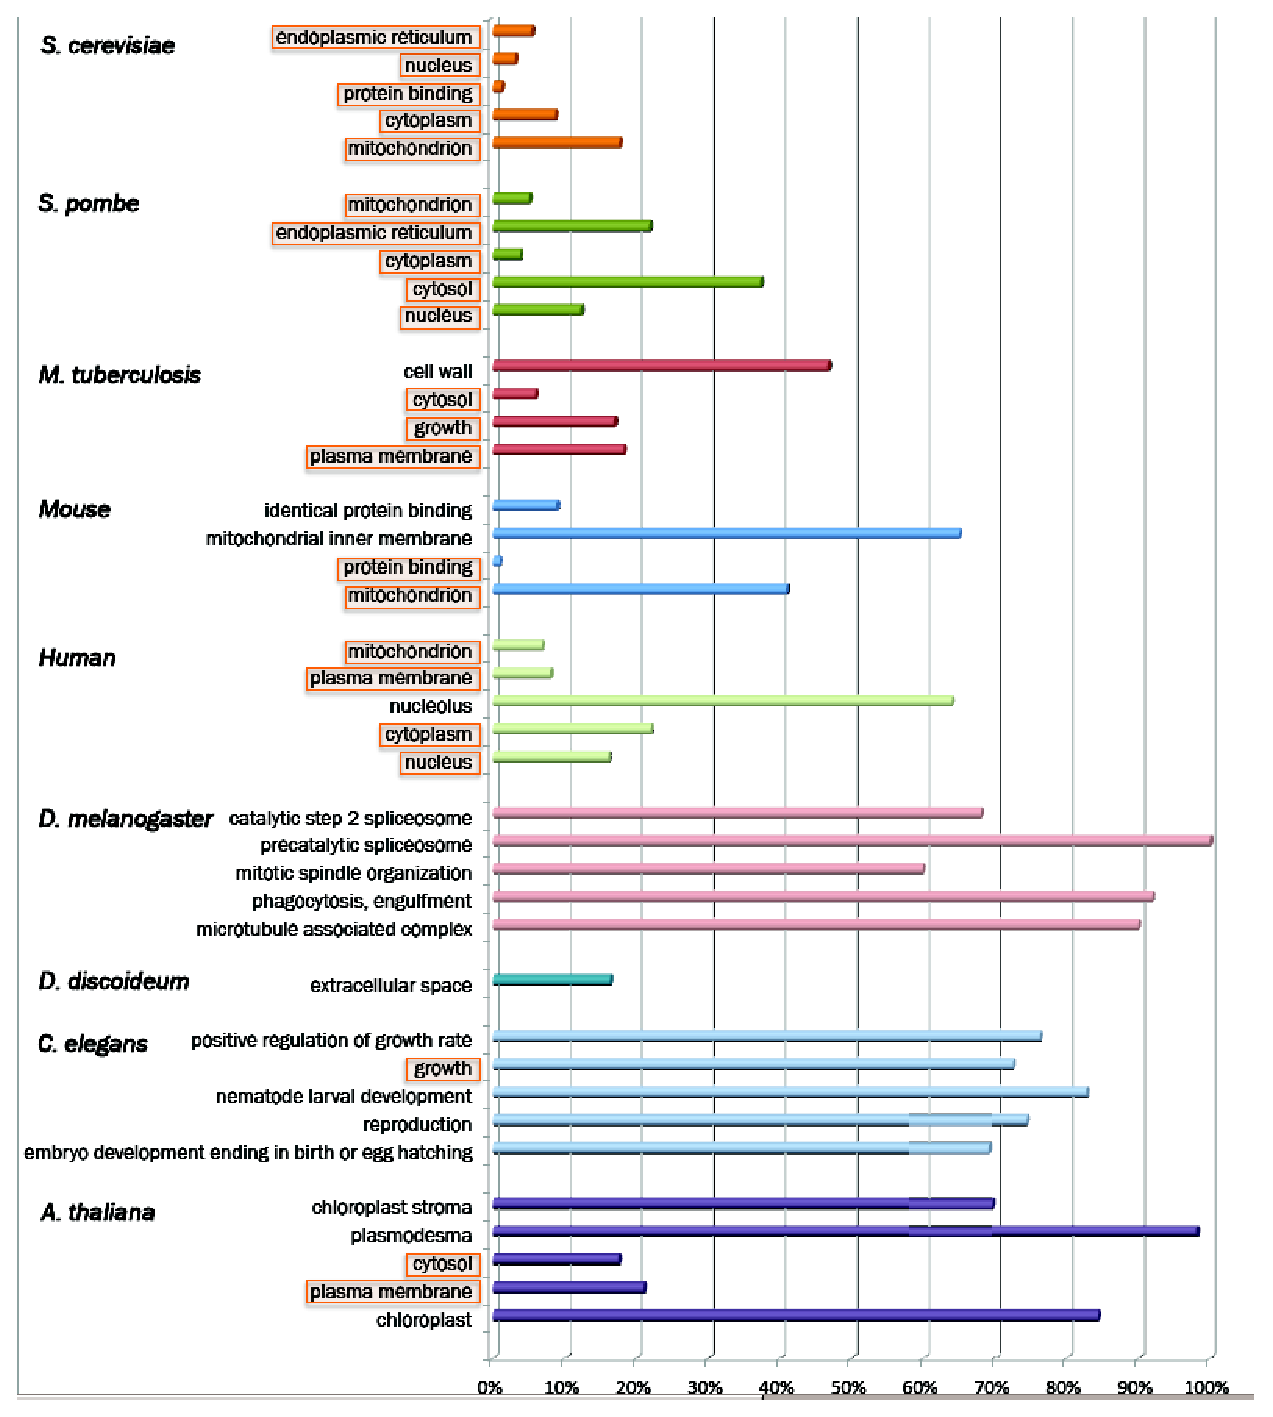
\includegraphics[width=6in]{rel-contrib.eps}
\end{center}
\caption{
{\bf Relative contribution of top-50 articles to the annotation of major model organisms.}  
The length of each bar represents the percentage of proteins annotated by the top-50 articles in a
given organism by a given GO term.
}
\label{fig:rel-contrib}
\end{figure}
\newpage

\begin{figure}[!ht]
\begin{center}
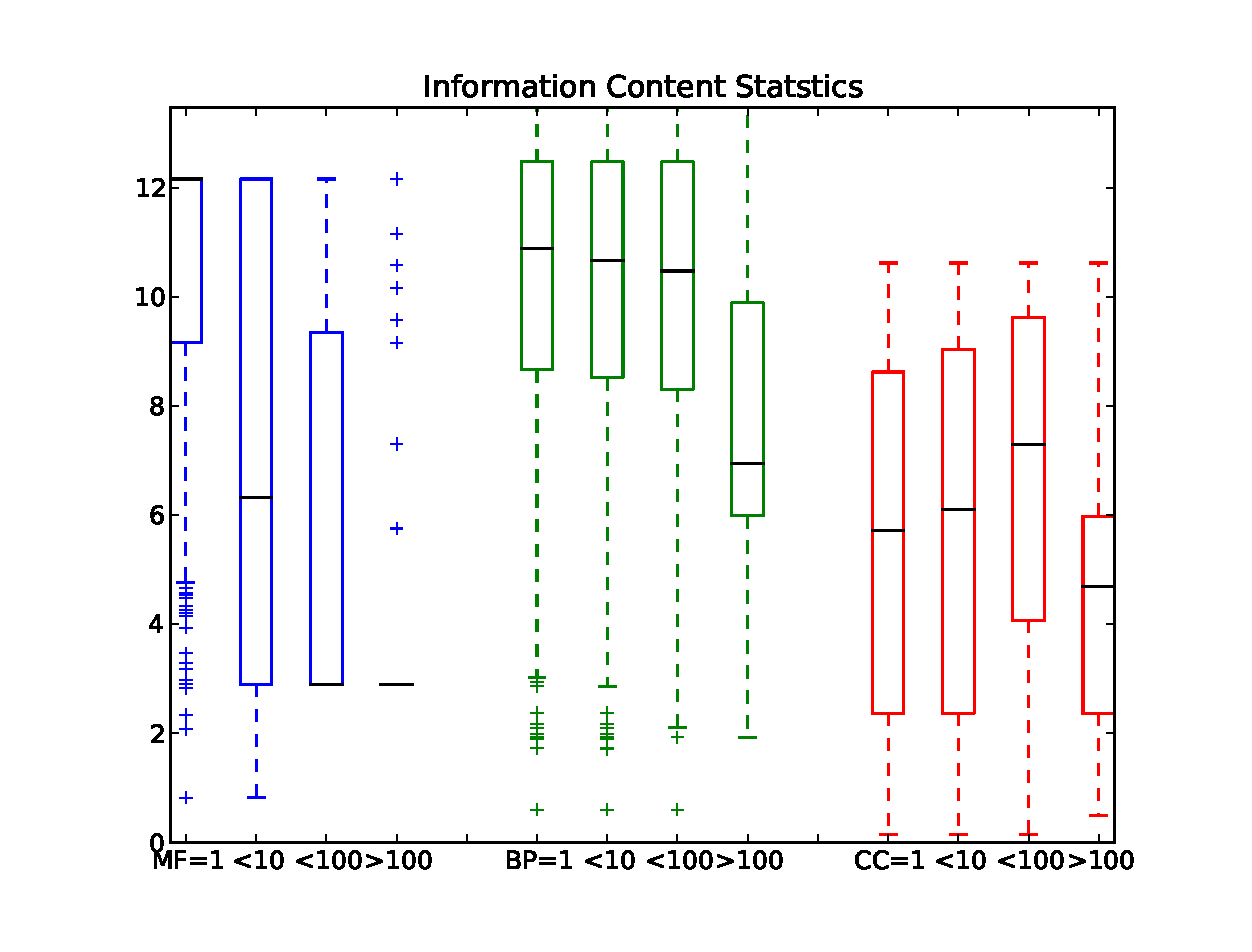
\includegraphics[width=6in]{boxplots-IC.eps}
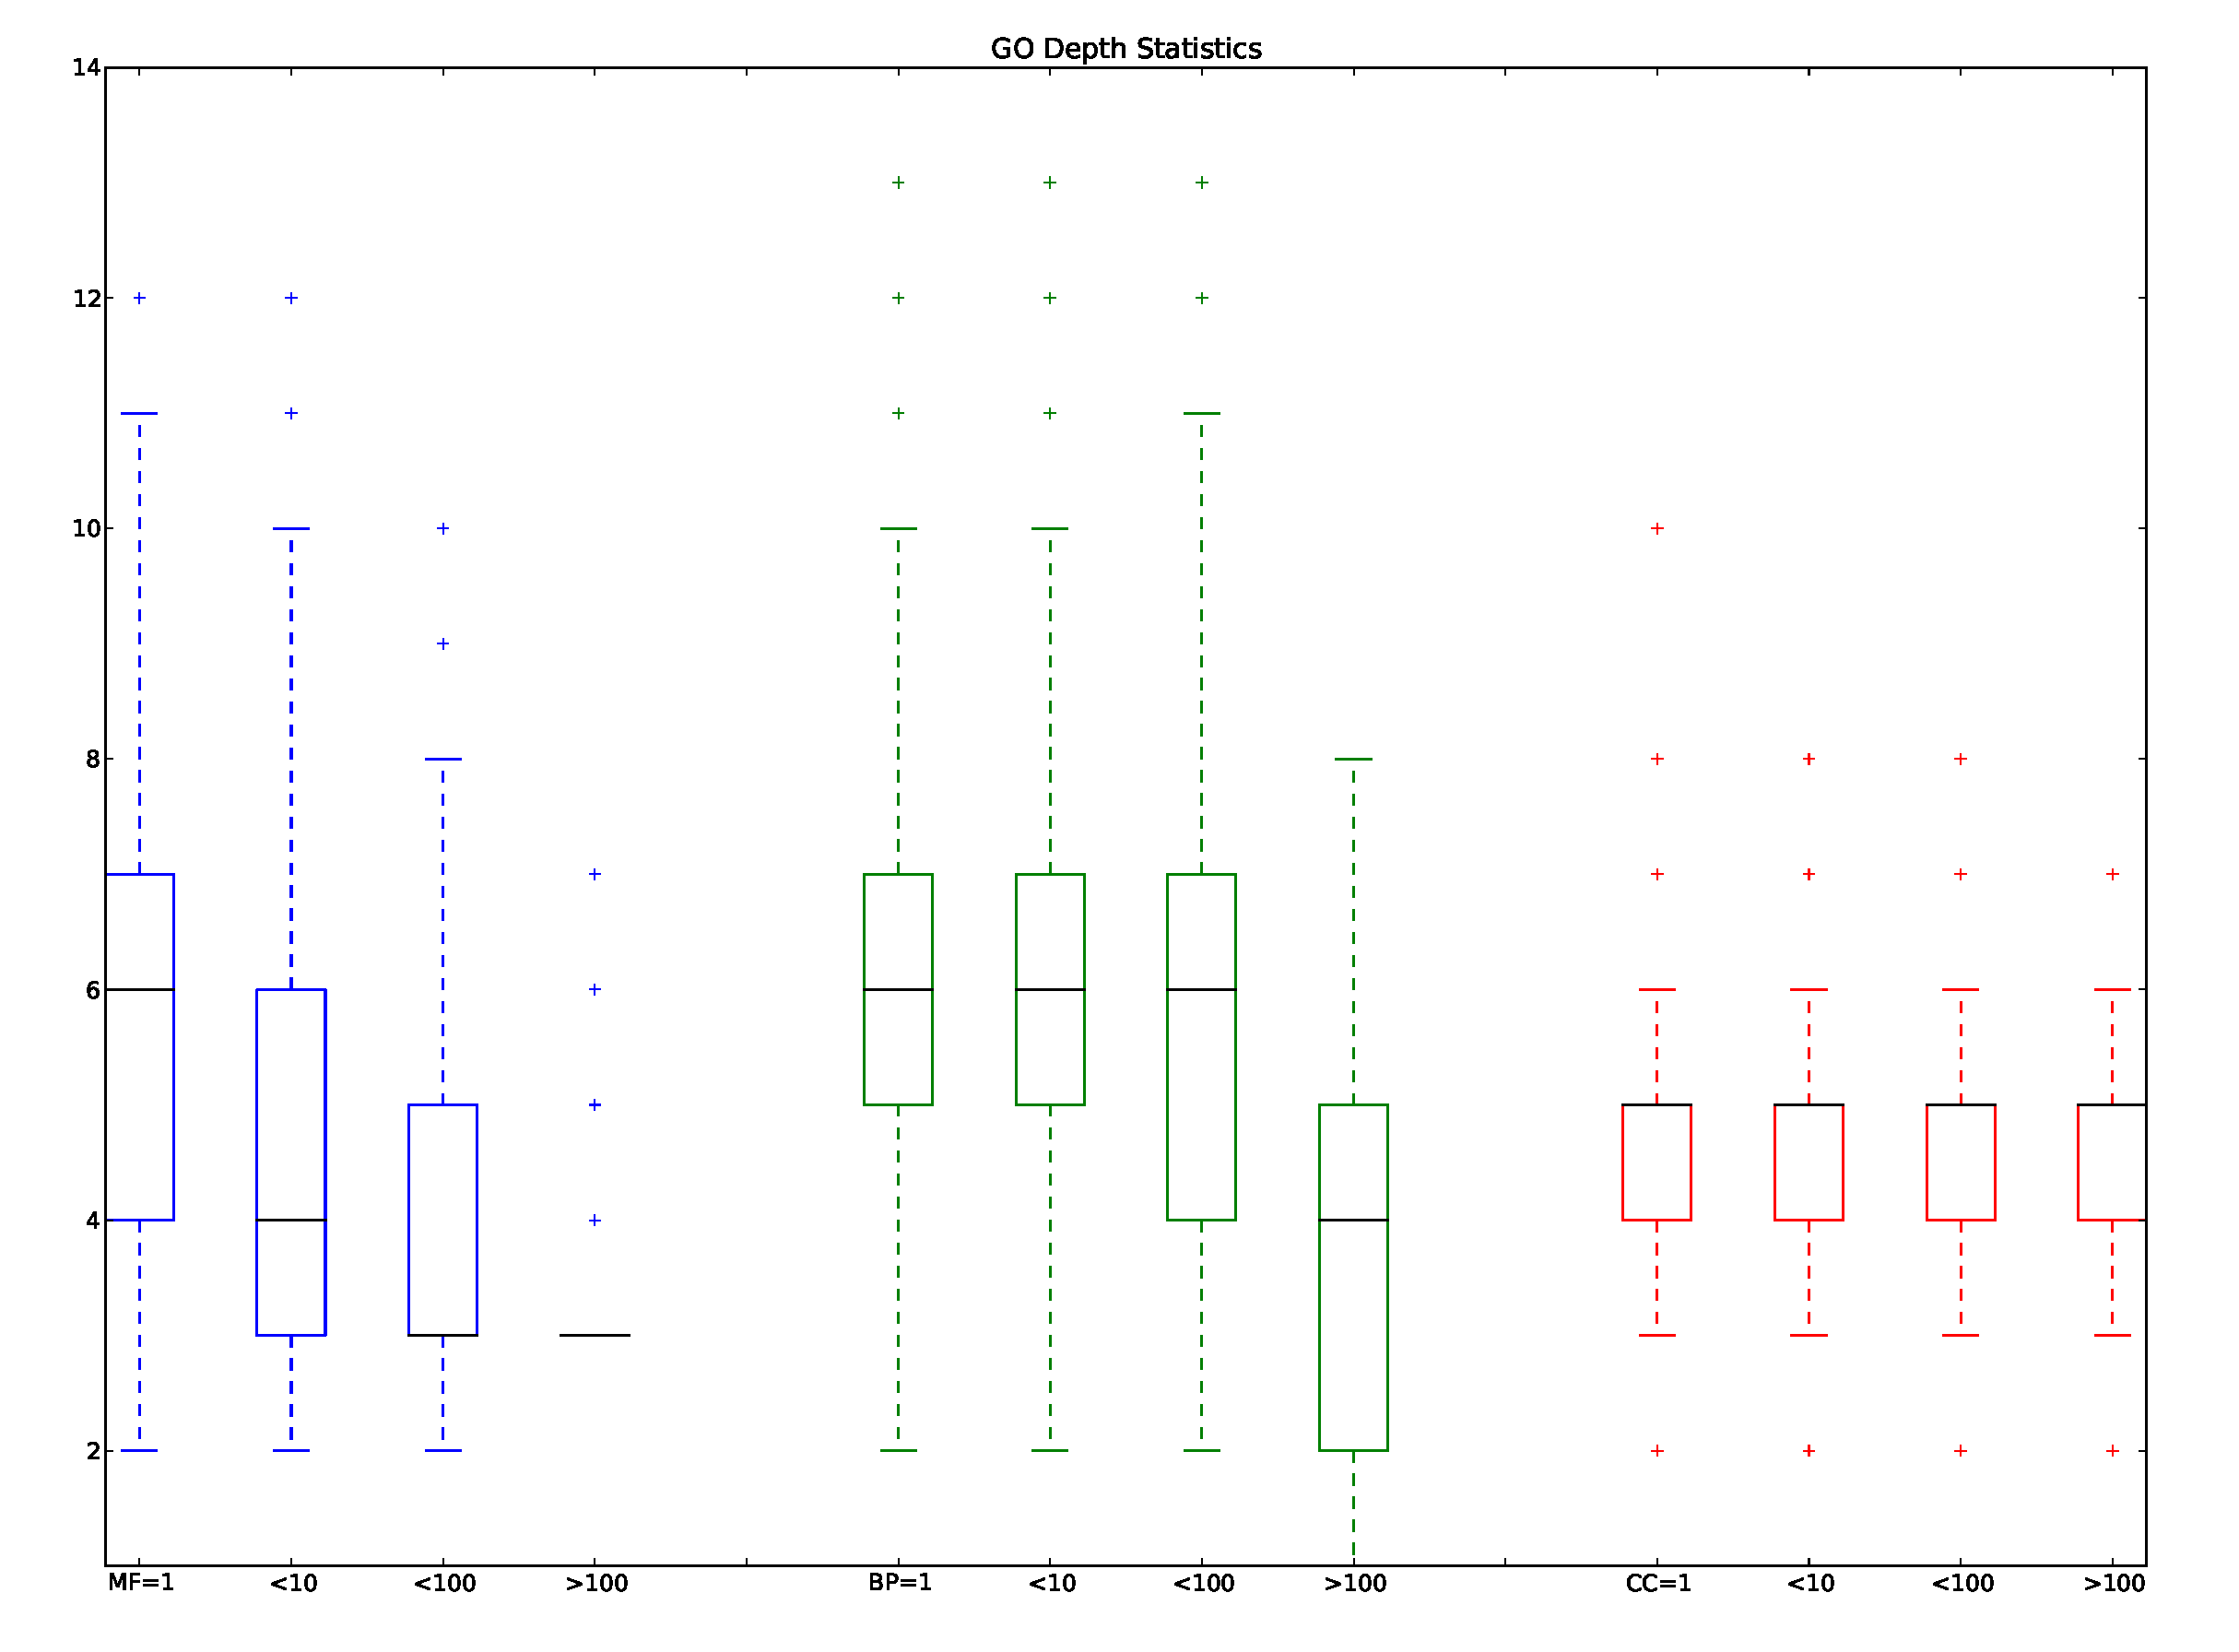
\includegraphics[width=5in]{boxplots-GOdepth.eps}
\end{center}
\caption{
{\bf Information provided by articles depending on the number of proteins the articles annotate.}
Articles are grouped into cohorts: 1: one protein annotated by article; <10: more than 1, less than 10
annotated; <100: more than 10, less than 100 annotated; $\ge 100$: more than 100 proteins annotated per
article. Blue bars: Molecular Function ontology; Green bars: Biological Process ontology; Red bars:
Cellular Component ontology. Information is gauged by {\bf A}: Information Content and{\bf B}: GO depth.
See text for details.}
\label{fig:rel-contrib}
\end{figure}
%\newpage
\clearpage

\section*{Tables}
%\begin{table}[!ht]
%\caption{
%\bf{Table title}}
%\begin{tabular}{|c|c|c|}
%table information
%\end{tabular}
%\begin{flushleft}Table caption
%\end{flushleft}
% \end{table}
% top 50 table
\begin{table}[!ht]
\caption{
\bf{Annotation Cohorts}}
\begin{tabular}{||p{5cm}||l|l|l|l||l||}
\hline
Articles annotating the following number of proteins & 1 & $1<n\le 10$ & $10<n\le 100$ & $n>100$ 
& SUM \\ \hline
\textbf{Number of proteins annotated} & 20699 & 46383 & 26485 & 31411 & 124978 \\ \hline
\textbf{Number of annotating articles} & 41156 & 32201 & 2668 & 62 &  76087 \\ \hline
\textbf{Percent of proteins annotated} & 16.56 & 37.11 & 21.19 & 25.13 & 100 \\ \hline
\textbf{Percent of annotating articles} & 54.09 & 42.32 & 3.51 & 0.08 & 100 \\ \hline 
\end{tabular}
\begin{flushleft}Table caption
\end{flushleft}
\label{tab:cohorts}
\end{table}
\newpage

\begin{longtable}[!ht]{|l|l|l|l|l|l|l|l|}
\caption{\textbf{Top 50 Annotating Articles}} \\
\hline
\textbf{N}&\textbf{Proteins}&\textbf{Annotations}&\textbf{Species}&
\textbf{ref.}&
\textbf{MFO}& \textbf{BPO}&\textbf{CCO}\\\hline
\endfirsthead
\hline
\textbf{N}&\textbf{Proteins}&\textbf{Annotations}&\textbf{Species}&
\textbf{ref.} &
\textbf{MFO}&\textbf{BPO}&\textbf{CCO} \\\hline
\endhead
\hline \multicolumn{4}{r}{\textit{Continued on next page}} \\
\endfoot
\hline
\endlastfoot
1 & 4937 & 11050 & \textit{H. sapiens} & \cite{pmid18029348} & 0 & 0 & 11050\\ \hline
2 & 4247 & 7046 & \textit{S. pombe} & \cite{pmid16823372} & 0 & 0 & 7046\\ \hline
3 & 2412 & 2412 & \textit{H. sapiens} & \cite{pmid18614015} & 0 & 0 & 2412\\ \hline
4 & 1791 & 5918 & \textit{C. elegans} & \cite{pmid14551910} & 0 & 5918 & 0\\ \hline
5 & 1406 & 1863 & \textit{S. cerevisiae} & \cite{pmid14562095} & 0 & 0 & 1863\\ \hline
6 & 1251 & 1251 & \textit{A. thaliana} & \cite{pmid18431481} & 0 & 0 & 1251\\ \hline
7 & 1205 & 1476 & \textit{C. elegans} & \cite{pmid15791247} & 0 & 1476 & 0\\ \hline
8 & 1186 & 1213 & \textit{M. musculus} & \cite{pmid14651853} & 0 & 0 & 1213\\ \hline
9 & 1136 & 1136 & \textit{A. thaliana} & \cite{pmid17317660} & 0 & 0 & 1136\\ \hline
10 & 1101 & 2269 & \textit{C. elegans} & \cite{pmid12529635} & 0 & 2269 & 0\\ \hline
11 & 1043 & 1365 & \textit{M. tuberculosis} & \cite{pmid15525680} & 0 & 0 & 1365\\ \hline
12 & 1041 & 1041 & \textit{A. thaliana} & \cite{pmid21166475} & 0 & 0 & 1041\\ \hline
13 & 865 & 1533 & \textit{C. elegans} & \cite{pmid15489339} & 0 & 1533 & 0\\ \hline
14 & 845 & 845 & \textit{S. cerevisiae} & \cite{pmid16823961} & 0 & 0 & 845\\ \hline
15 & 784 & 784 & \textit{A. thaliana} & \cite{pmid21533090} & 0 & 0 & 784\\ \hline
16 & 735 & 735 & \textit{M. tuberculosis} & \cite{pmid14532352} & 0 & 0 & 735\\ \hline
17 & 724 & 882 & \textit{A. thaliana} & \cite{pmid20061580} & 0 & 0 & 882\\ \hline
18 & 634 & 634 & \textit{A. thaliana} & \cite{pmid15028209} & 0 & 0 & 634\\ \hline
19 & 613 & 613 & Mycobacter sp. & \cite{pmid12657046} & 0 & 613 & 0\\ \hline
20 & 607 & 661 & \textit{C. elegans} & \cite{pmid17704769} & 0 & 659 & 2\\ \hline
21 & 577 & 577 & \textit{A. thaliana} & \cite{pmid17432890} & 0 & 0 & 577\\ \hline
22 & 553 & 884 & \textit{C. elegans} & \cite{pmid11231151} & 0 & 884 & 0\\ \hline
23 & 516 & 5972 & \textit{C. elegans} & \cite{pmid17417969} & 0 & 5972 & 0\\ \hline
24 & 503 & 503 & \textit{S. cerevisiae} & \cite{pmid14576278} & 0 & 0 & 503\\ \hline
25 & 498 & 638 & \textit{S. cerevisiae} & \cite{pmid16429126} & 638 & 0 & 0\\ \hline
26 & 479 & 848 & \textit{C. elegans} & \cite{pmid21529718} & 0 & 848 & 0\\ \hline
27 & 465 & 468 & \textit{H. sapiens} & \cite{pmid11256614} & 0 & 0 & 468\\ \hline
28 & 436 & 436 & \textit{A. thaliana} & \cite{pmid17644812} & 0 & 0 & 436\\ \hline
29 & 430 & 513 & \textit{A. thaliana} & \cite{pmid16618929} & 0 & 0 & 513\\ \hline
30 & 413 & 456 &  \textit{D. melanogaster} & \cite{pmid18433294} & 0 & 39 & 417\\ \hline
31 & 401 & 401 & \textit{A. thaliana} & \cite{pmid17151019} & 0 & 0 & 401\\ \hline
32 & 392 & 392 & \textit{A. thaliana} & \cite{pmid14671022} & 0 & 0 & 392\\ \hline
33 & 392 & 639 & \textit{C. elegans} & \cite{pmid12529643} & 0 & 639 & 0\\ \hline
34 & 383 & 917 & \textit{C. elegans} & \cite{pmid12445391} & 0 & 917 & 0\\ \hline
35 & 380 & 380 & \textit{A. thaliana} & \cite{pmid15539469} & 0 & 0 & 380\\ \hline
36 & 375 & 375 & \textit{M. musculus} & \cite{pmid12865426} & 0 & 0 & 375\\ \hline
37 & 343 & 509 & \textit{H. sapiens} & \cite{pmid16189514} & 509 & 0 & 0\\ \hline
38 & 338 & 338 & Ddiscoideum & \cite{pmid20422638} & 0 & 0 & 338\\ \hline
39 & 328 & 328 & \textit{A. thaliana} & \cite{pmid12938931} & 0 & 0 & 328\\ \hline
40 & 319 & 329 & \textit{C. albicans} & \cite{pmid16336044} & 1 & 328 & 0\\ \hline
41 & 305 & 312 & \textit{A. thaliana} & \cite{pmid18633119} & 0 & 0 & 312\\ \hline
42 & 290 & 331 & \textit{S. cerevisiae} & \cite{pmid11914276} & 0 & 0 & 331\\ \hline
43 & 285 & 761 & \textit{C. elegans} & \cite{pmid11099033} & 0 & 761 & 0\\ \hline
44 & 283 & 499 & \textit{C. elegans} & \cite{pmid11099034} & 0 & 499 & 0\\ \hline
45 & 266 & 433 & \textit{M. musculus} & \cite{pmid11591653} & 433 & 0 & 0\\ \hline
46 & 260 & 260 & \textit{A. thaliana} & \cite{pmid16502469} & 0 & 260 & 0\\ \hline
47 & 258 & 259 & \textit{S. pombe} & \cite{pmid12529438} & 0 & 259 & 0\\ \hline
48 & 244 & 397 &  \textit{D. melanogaster} & \cite{pmid17412918} & 0 & 367 & 30\\ \hline
49 & 242 & 397 &  \textit{D. melanogaster} & \cite{pmid18981222} & 0 & 0 & 397\\ \hline
50 & 241 & 263 & \textit{A. thaliana} & \cite{pmid16287169} & 0 & 0 & 263\\ \hline
\end{longtable}
%\end{tabular}
\begin{flushleft} {\bf The top 50 annotating articles.} \textbf{N}:
article rank; \textbf{Proteins}: number of proteins annotated in this
article; \textbf{Annotations}: number of annotating
GO terms; \textbf{Species}: annotated species; \textbf{ref.} annotating
article; \textbf{MFO}/\textbf{BPO}/\textbf{CCO}: number of proteins
annotated in the Molecular Function, Biological Process and Cellular
Component ontologies, respectively.
\end{flushleft}

\label{tab:top50}
\newpage


\begin{table}[!ht]
\caption{
\bf{Sequence Redundancy in Top-50 Annotating Articles}}
\begin{tabular}{|p{3cm}|p{1.5cm}|p{2cm}|p{2cm}|p{2cm}|p{2cm}|} %p{2cm}|p{2cm}|}
\hline
\textbf{Species} & \textbf{num. articles} &\textbf{num. prot} & \textbf{Clusters at 100\%} & 
\textbf{\% redundancy} & \textbf{Mean genes/ cluster} % & \textbf{\% redundancy, norm.}  
% & \textbf{Clusters at 95\%} & \textbf{\% redundancy} 
\\ \hline
\textit{C. elegans}  & 12 & 8416 & 3338 & 60 & 3.74 %& 5.0 & %& 3292 & 61\% 
\\ \hline
\textit{A. thaliana}  & 16 &  8879 & 4694 & 47 & 3.92 %& 3.21 %& 4595 & 48\% \
\\ \hline
\textit{M. musculus}  & 3 &  4220 & 2273 & 46 & 2.75  %& 15.33 %& 1813 & 57\% 
\\ \hline
\textit{M. tuberculosis}  & 2 & 2351& 1702& 28 & 2.22 %& 14.0 %& 1700 & 28\% 
\\ \hline
\textit{S. cerevisiae}  & 5 & 3542 & 2550 & 28 & 2.33 %& 5.6 %& 2546 & 28\% 
\\ \hline
\textit{H. sapiens}  & 4 & 5593 & 4509 & 19 & 2.36 %& 4.75 %& 3748 & 33\% 
\\ \hline
\textit{D. melanogaster} & 3  & 1217 & 1003 & 18 & 2.17 %&  6.0 % & 767 & 37\% 
\\ \hline
\textit{S. pombe}  & 2 & 4502 & 4281 & 5 & 2.00 %& 2.5 %& 4253 & 6\% 
\\ \hline
\end{tabular}
\begin{flushleft} 
\textbf{Species}: annotated species; 
\textbf{num. articles} number of annotating articles;
\textbf{num. prot}: number of proteins annotated by top-50 articles for that species; 
\textbf{Clusters at 100\%}: number of clusters of 100\% identical proteins; 
\textbf{\% redundancy}: the ratio between column 3 and column 2: this is the percentage of proteins
annotated more than once for a given species in the top 50 articles; 
\textbf{Mean genes/cluster}: the mean number of genes per cluster, for clusters
having more than a single gene.
\end{flushleft}
\label{tab:dreamcatcher1}
\end{table}
\newpage

\begin{table}[!ht]
% Generated using Uniprot-Bias/SameAnnotationData/annot_consistency.py
\caption{
\bf{Annotation Consistency in Top 50 articles}}
\begin{tabular}{|p{3cm}|l|l|l|l|l|l|l|}
\hline
\textbf{Species} & \textbf{Ontology} & \textbf{num prot} & \textbf{mean} 
$k_{P,O}$ &
\textbf{stdv} & \textbf{stderr} & \textbf{num articles} & \textbf{num terms} \\
\hline \hline
% A. thaliana & bpo & 207 & 0 & 0 & 0 & 1 & 1\\ \hline
A. thaliana & cco & 1941 & 0.251 & 0.328 & 0.007 & 15 & 18\\ \hline\hline
C. elegans & bpo & 1847 & 0.388 & 0.239 & 0.006 & 12 & 41\\ \hline 
%C. elegans & cco & 2 & 0 & 0 & 0 & 1 & 1\\ \hline\hline
D. melanogaster & bpo & 76 & 0.086 & 0.22 & 0.025 & 3 & 8\\ \hline
D. melanogaster & cco & 81 & 0.068 & 0.234 & 0.026 & 3 & 5\\ \hline\hline
%H. sapiens & mfo & 89 & 0.17 & 0.367 & 0.039 & 1 & 2\\ \hline
H. sapiens & cco & 167 & 0.285 & 0.365 & 0.028 & 2 & 20\\ \hline\hline
%M. musculus & mfo & 11 & 0.114 & 0.247 & 0.074 & 1 & 2\\ \hline
M. musculus & cco & 807 & 0.832 & 0.291 & 0.01 & 3 & 2\\ \hline\hline
%S. pombe & bpo & 221 & 0 & 0 & 0 & 1 & 4\\ \hline
%S. pombe & cco & 221 & 0 & 0 & 0 & 1 & 12\\ \hline\hline
%S. cerevisiae & mfo & 163 & 0.123 & 0.328 & 0.026 & 1 & 1\\ \hline
S. cerevisiae & cco & 744 & 0.759 & 0.379 & 0.014 & 4 & 15\\ \hline\hline
%B. tuberculosis & bpo & 328 & 0 & 0 & 0 & 1 & 1\\ \hline
B. tuberculosis & cco & 532 & 0.309 & 0.41 & 0.018 & 2 & 3\\ \hline\hline
\end{tabular}
\begin{flushleft}
\textbf{Species}: annotated species;
\textbf{Ontology}: annotating GO ontology;
\textbf{num prot}: number of annotated proteins in that species \& ontology that are annotated by
more than one paper.
\textbf{mean, stdv, stderr}: mean number of consistent annotations for a protein in that species
and ontology. Standard deviation form the mean and standard error are also provided.
\textbf{num articles}: number of annotating articles
\textbf{num terms} number of annotating terms. 
Annotations by less than 2 articles or two terms (or both) for the same protein/ongology
combination have been omitted.
\end{flushleft}
\label{tab:dreamcatcher2}
\end{table}
\newpage
%%\begin{table}[!ht]
%%% Generated using Uniprot-Bias/SameAnnotationData/annot_consistency.py
%%\caption{
%%\bf{Annotation Consistency in Top 50 articles}}
%%\begin{tabular}{|p{3cm}|l|l|l|l|l|l|l|}
%%\hline
%%Species & Ontology & Nclust & Mean & Stdv & Stderr & Narticles & Nterms \\ \hline
%%\textit{A. thaliana} & BPO & 0 & 0 & 0 & 0 & 1 & 1 \\ \hline
%%\textit{A. thaliana} & CCO & 1883 & 0.082 & 0.271 & 0.006 & 15 & 18 \\ \hline
%%\textit{C. elegans} & BPO & 1847 & 0.127 & 0.258 & 0.006 & 12 & 41 \\ \hline
%%\textit{C. elegans} & CCO & 0 & 0 & 0 & 0 & 1 & 1 \\ \hline
%%\textit{D. melanogaster} & BPO & 15 & 0.3 & 0.245 & 0.063 & 3 & 8 \\ \hline
%%\textit{D. melanogaster} & CCO & 15 & 0 & 0 & 0 & 3 & 5 \\ \hline
%%\textit{H. sapiens} & MFO & 0 & 0 & 0 & 0 & 1 & 2 \\ \hline
%%\textit{H. sapiens} & CCO & 83 & 0.325 & 0.36 & 0.04 & 2 & 20 \\ \hline
%%\textit{M. musculus} & MFO & 0 & 0 & 0 & 0 & 1 & 2 \\ \hline
%%\textit{M. musculus} & CCO & 800 & 0.672 & 0.469 & 0.017 & 3 & 2 \\ \hline
%%\textit{S. pombe} & BPO & 0 & 0 & 0 & 0 & 1 & 4 \\ \hline
%%\textit{S. pombe} & CCO & 0 & 0 & 0 & 0 & 1 & 12 \\ \hline
%%\textit{S. cerevisiae} & MFO & 0 & 0 & 0 & 0 & 1 & 1\\ \hline
%%\textit{S. cerevisiae} & CCO & 635 & 0.796 & 0.383 & 0.015 & 4 & 15\\ \hline
%%\textit{B. tuberculosis} & MFO & 0 & 0 & 0 & 0 & 0 & 0\\ \hline
%%\textit{B. tuberculosis} & BPO & 0 & 0 & 0 & 0 & 1 & 1\\ \hline
%%\textit{B. tuberculosis} & CCO & 321 & 0.457 & 0.41 & 0.023 & 2 & 3\\ \hline
%%\end{tabular}
%%\begin{flushleft}Table caption
%%\end{flushleft}
%%\label{tab:dreamcatcher2}
%%\end{table}

\begin{longtable}[!ht]{|l||l|p{8cm}|l|}
\caption{\textbf{Count of ECO terms in top-50 papers}} \\
\hline
\textbf{N} & \textbf{ECO id} & \textbf{ECO term} & \textbf{Articles} \\ \hline
\endfirsthead
\hline
\textbf{N} & \textbf{ECO id} & \textbf{ECO term} & \textbf{Articles} \\ \hline
\endhead
\hline
\multicolumn{4}{r}{\textit{Continued on next page}} \\
\endfoot
\hline
\endlastfoot
1 & ECO:0000160 & protein separation followed by fragment identification evidence & 25\\ \hline
2 & ECO:0000004 & cell fractionation evidence & 21\\ \hline
3 & ECO:0000053 & \textbf{computational combinatorial evidence} & 18\\ \hline
4 & ECO:0000249 & \textbf{sequence similarity evidence used in automatic assertion} & 18\\ \hline
5 & ECO:0000315 & mutant phenotype evidence used in manual assertion & 16\\ \hline
6 & ECO:0000019 & RNAi experimental evidence & 15\\ \hline
7 & ECO:0000028 & \textbf{motif similarity evidence} & 14\\ \hline
8 & ECO:0000112 & Western blot evidence & 9\\ \hline
9 & ECO:0000081 & targeting sequence prediction evidence & 7\\ \hline
10 & ECO:0000083 & transmembrane domain prediction evidence & 5\\ \hline
11 & ECO:0000126 & GFP fusion protein localization evidence & 5\\ \hline
12 & ECO:0000250 & \textbf{sequence similarity evidence used in manual assertion} & 4\\ \hline
13 & ECO:0000031 & \textbf{protein BLAST evidence used in manual assertion} & 4\\ \hline
14 & ECO:0000044 & \textbf{sequence similarity evidence} & 4\\ \hline
15 & ECO:0000104 & microarray RNA expression level evidence & 3\\ \hline
16 & ECO:0000245 & \textbf{computational combinatorial evidence used in manual assertion} & 3\\ \hline
17 & ECO:0000015 & transposon integration & 2\\ \hline
18 & ECO:0000128 & YFP fusion protein localization evidence & 2\\ \hline
19 & ECO:0000092 & epitope-tagged protein immunolocalization evidence & 2\\ \hline
20 & ECO:0000007 & immunofluorescence evidence & 2\\ \hline
21 & ECO:0000248 & \textbf{sequence alignment evidence used in automatic assertion} & 1\\ \hline
22 & ECO:0000010 & protein expression evidence & 1\\ \hline
23 & ECO:0000231 & qRT-PCR evidence & 1\\ \hline
24 & ECO:0000122 & protein localization evidence & 1\\ \hline
25 & ECO:0000181 & \textit{in-vitro} assay evidence & 1\\ \hline
26 & ECO:0000208 & \textbf{protein BLAST evidence} & 1\\ \hline
27 & ECO:0000108 & reverse transcription polymerase chain reaction transcription evidence & 1\\ \hline
28 & ECO:0000062 & genomic microarray evidence & 1\\ \hline
29 & ECO:0000106 & Northern assay evidence & 1\\ \hline
30 & ECO:0000026 & nucleic acid hybridization evidence & 1\\ \hline
31 & ECO-0000068 & yeast 2-hybrid evidence & 1\\ \hline
32 & ECO:0000176 & mutant visible phenotype evidence & 1\\ \hline
33 & ECO:0000324 & imaging assay evidence & 1\\ \hline
34 & ECO:0000079 & affinity chromatography evidence & 1\\ \hline
35 & ECO:0000022 & co-purification evidence & 1\\ \hline
36 & ECO:0000266 & \textbf{sequence orthology evidence used in manual assertion} & 1\\ \hline
37 & ECO:0000025 & hybrid interaction evidence & 1\\ \hline
38 & ECO:0000124 & RFP fusion protein localization & 1\\ \hline
\end{longtable}
\label{tab:assertion}
\begin{flushleft} ECO terms were assigned by the authors to the top-50 annotating papers. The table entries are
ranked by the frequency of the assignments, i.e. 25 papers are assigned with term ECO:0000160, 21 were
assigned ECO:0000004, etc. Entries in \textbf{boldface} are for computational methods, which were used in
many papers in combination with experimental methods to assign function. 
\end{flushleft}

\end{document}
